\documentclass[12pt,a4paper]{report}
\usepackage[T1]{fontenc}
\usepackage[utf8]{inputenc}
\usepackage{graphicx} 

\begin{document}

\begin{titlepage}
\begin{center}

\includegraphics[scale=0.5]{IMG/upx.png} \vspace{2cm} 
\newline
\textsc{\Large Rapport de stage}\\[0.5cm] 
\hrule 
{\huge \vspace{0.4cm}\bfseries Développeur informatique\par}\vspace{0.4cm}
\hrule 
\vspace{0.6cm}\emph{Réalisé par Mamadou Baba MAKADJI \newline étudiant Master 1 MIAGE 2016 - 2017}\vspace{2cm}
\newline
\begin{minipage}[t]{0.4\textwidth}
\begin{flushleft} \large
\emph{Responsable de formation:} \\ Pascal POIZAT
\end{flushleft}
\end{minipage}
\begin{minipage}[t]{0.4\textwidth}
\begin{flushright} \large
\emph{Enseignant référent :} \\ Sonia GUEHIS
\end{flushright}
\end{minipage}\\[2cm]
\textsc{\Large Organisme d'accueil}\\[0.5cm] 

\includegraphics[scale=0.5]{IMG/amundi.jpg} \\[0.5cm]
\textbf{Période} : 03 Avril 2017 au 18 Août 2017 \vspace{0.4cm}
\newline
\emph{Maître de stage :} \\ Frank GILLES \vspace{0.3cm}
(Responsable équipe IT Conformité)
\end{center}
\end{titlepage}

\newpage
\begin{center} \textbf{\Large Remerciements} \vspace{2cm} \end{center} 

Je tiens tout d'abord à remercier Franck GILLES, mon maître de stage, pour m'avoir accepté en tant que stagiaire au sein de Amundi IT Services et m'avoir accordé sa confiance dans les projets qui m'ont été confiés.
Je tiens également à remercier Wajdi BEN SLIMANE, Gregoire SUPPLY, Adrien JOURDAN pour leur soutien technique.
Je tiens aussi à les remercier pour m'avoir intégré très rapidement au sein de leur équipe, pour tous leurs conseils qui ont été précieux et qui m'ont permis de mener mes missions à bien.\vspace{0.6cm}
\newline
Pour toutes ces raisons je remercie Amundi IT Services pour m'avoir permis de réaliser cette nouvelle expérience professionnelle, ainsi que l'équipe pédagogique  de la formation Méthodes Informatiques Appliquées à la Gestion des Entreprises (MIAGE) pour leur apprentissage tant théorique que pratique qui m'a permis de réaliser les missions que j'ai eues. \vspace{0.6cm}
\newline
J'ai été ravi d'effectuer mon stage au sein de Amundi IT Services, cela m'a conforté dans mon projet professionnel.

\newpage
\begin{center} \textbf{\Large Introduction} \vspace{2cm} \end{center} 

Actuellement en Master 1 MIAGE à l’Université Paris Ouest Nanterre la Défense, il est de coutume de valider le cursus par une immersion dans le monde professionnel. L’objectif de ce stage est de mettre en pratique les connaissances acquises tout au long de la formation sur un aspect informatique.
\vspace{0.5cm}
\newline
Ayant toujours été attiré par le domaine bancaire, je me suis orienté vers un stage au sein de Amundi Asset Management, filiale du Crédit Agricole  afin de me faire une idée plus précise de ce que peut apporter l’informatique à la banque et, plus précisement, dans le domaine de la gestion d'actifs et de la conformité. J’ai donc eu l’opportunité de pouvoir évoluer au sein de cette entreprise durant 18 semaines dans l'équipe IT de la conformité.\newline
Amundi est un acteur mondial de la gestion d'actifs avec 1128 milliards d'euros d'actifs sous gestion au plan mondial, Amundi est le premier Asset Manager européen.\vspace{0.5cm} \newline
Ma mission consiste à mener à bien des migrations techniques (migration Ant vers Maven, …), à faire des préconisations afin d’améliorer la qualité des développements des applicatifs optimisant et factorisant le code existant (Java, SQL).\newline J'ai été également amené à contribuer aux projets, évolutions et correctifs liés à l'activité, mais aussi à la revue et l’amélioration du socle applicatif existant.\newline Afin de mener à bien ma mission, j'ai eu l'occasion d'utiliser les langages de programmation(java, SQL), mais aussi divers outils(Eclipse, GIT, Jira...). 
\newline
Dans un premier temps, je présenterai l’entreprise Amundi et son organisation. Nous verrons ensuite les étapes de la réalisation du projet, puis je détaillerai les étapes concernant l’utilisation des langages et outils utilisés dans le cadre de ma mission. Enfin, je terminerai ce rapport en émettant un avis personnel sur les apports et les difficultés de cette expérience professionnelle.

\newpage
\renewcommand\contentsname{Sommaire}
\tableofcontents

\newpage
\section{\textbf{ Amundi Asset Management}}
\subsection{Présentation générale de l'entreprise}
Amundi est une entreprise de gestion d'actifs(asset management) née du rapprochement des expertises de gestion d'actifs de deux groupes bancaires puissants : Crédit Agricole et Société Générale. Amundi occupe des positions de premier plan en France et en Europe, et appuie son ambition de développement sur des relais solides à l'international.
Amundi est le premier gestionnaire d’actifs européen en termes d’encours, avec plus de 1 128 milliards d’euros sous gestion dans le monde.\vspace{0.6cm}

Présente dans plus de 30 pays, Amundi dispose de centres de gestion couvrant les principales places financières en Europe (Paris, Londres, Dublin, Milan), en Asie (Japon, Hong-Kong, Singapour), et aux Etats-Unis. Elle est également présente sur toutes les classes d’actifs et les grandes devises (Euro, Yen, Dollar, Sterling) et dispose d’un important département Recherche, Stratégie et Analyse.
\subsection{Principes généraux}
L’organisation d’Amundi a pour objectif de permettre un déploiement cohérent et efficace de sa stratégie au service de la clientèle des particuliers (« Retail ») et des institutionnels et corporate en France et à l’étranger.
\newline
Les composantes de l’organisation d’Amundi sont les suivantes :
\subsubsection{Deux pôles clients}
Retail et clientèle Institutionnelle. Ces deux pôles ont pour mission d’élaborer la stratégie commerciale et de concevoir les produits en liaison avec les lignes métier, et de les mettre en oeuvre sur chacun des segments. Les produits sont adaptés à chacun des canaux de distribution et à chaque pays.
\subsubsection{9 pôles métiers}
Ces pôles métier regroupent les plateformes de gestion et leurs forces commerciales spécifiques. Ils ont vocation à mettre en oeuvre les expertises de gestion identifiées par les pôles clients et à contribuer à leur promotion commerciale dans les cadres définis au sein des pôles clients.
\newline
\begin{tabular}{p{.3\textwidth}p{.5\textwidth}p{.9\textwidth}}
\flushleft 
\begin{itemize}
\item Fixed Income
\item Actions
\item ETF, Indiciel et smart beta
\end{itemize}
&\begin{center}
\begin{itemize}
\item Epargne Salariale
\item Produits structurés et garantis
\item Services Assuranciels
\end{itemize}
\end{center}
& \flushright
\begin{itemize}
\item Trésorerie
\item Gestions Diversifiées
\item Actifs Réels
\end{itemize}

\end{tabular}
Par ailleurs, deux entités, CPR AM et BFT IM disposent d’un statut spécifique caractérisé par une autonomie de leurs moyens commerciaux et d’équipes de gestion dédiées.

\subsubsection{Les plateformes de gestion}
Les métiers s’appuient sur les plateformes de gestion suivantes:
\begin{itemize}
\item Plateforme des gestions alpha : Fixed Income, Equities
\item Plateforme des gestions diversifiées et conseils: Gestions Diversifiées Retail et Epargne Salariale, Gestions Diversifiées institutionnels
\item Plateforme des gestions ETF, Indicielles et smart beta
\item Plateforme de gestions des produits de trésorerie
\item Plateforme des gestions structurées
\item Plateforme PARA : Immobilier, Dettes Privées, Private Equity, Infrastructures, Multigestion Private Markets et Alternatifs
\end{itemize}
Les plateformes de gestion inscrivent leur politique d’investissement et de gestion des risques dans le cadre des orientations définies dans les différents comités de politique d’investissement.
Elles bénéficient de l’appui du département d’analyse et de recherche et de la Table de négociation.
Le CIO d’Amundi (P. Blanqué) et son adjoint (V. Mortier) assurent l’encadrement de l’ensemble des plateformes de gestion en vue d’optimiser les performances dans un contexte de risque maîtrisé.
\newline
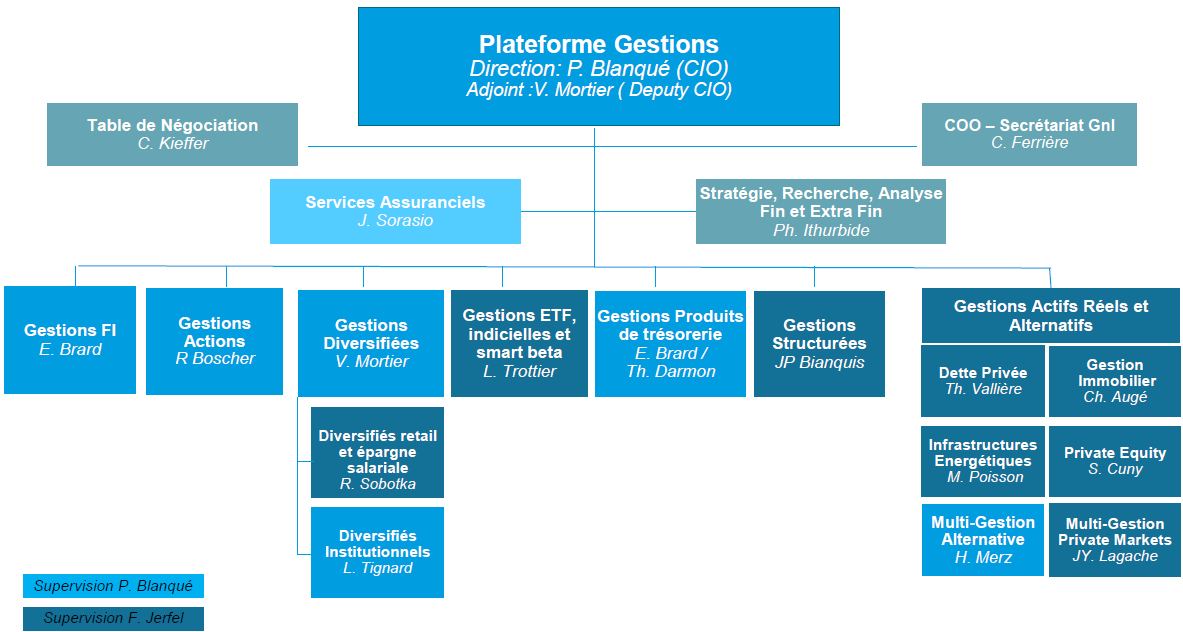
\includegraphics[scale=0.7]{IMG/orga.png} \\[0.5cm]
\subsubsection{Le pôle Pilotage et Contrôle (PCO)}
Il a pour missions d’assurer la conformité du fonctionnement d’Amundi au plan réglementaire, une bonne gestion des risques et une gestion financière efficace.
Il comprend les fonctions régaliennes suivantes : Finances, Risques, Juridique, Conformité, Inspection Générale. \vspace{0.5cm}
\newline
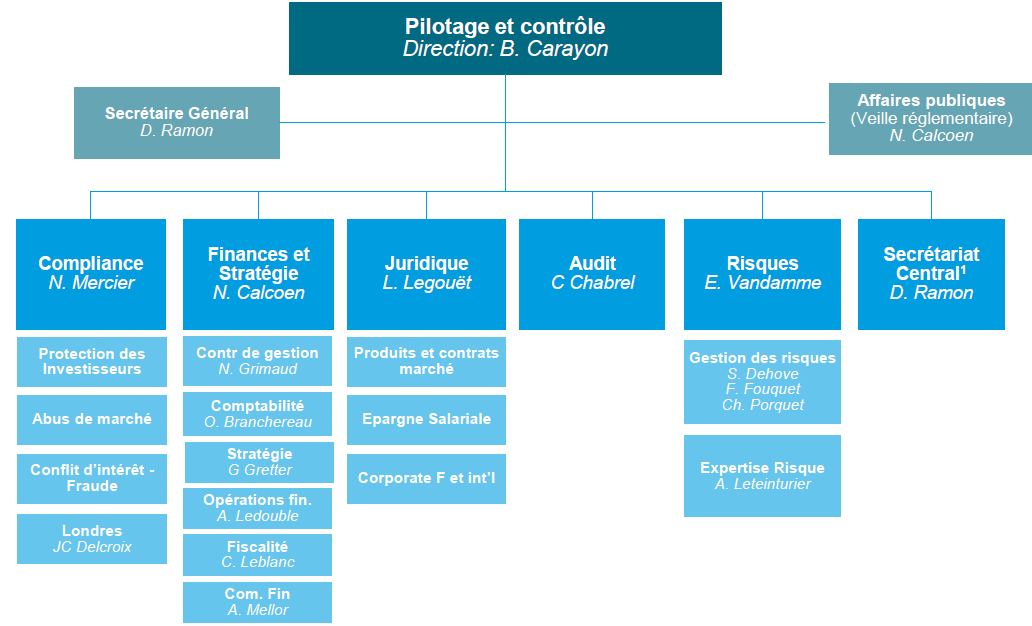
\includegraphics[scale=0.7]{IMG/orga2.png} 
\subsubsection{Le pôle Support et Développement (SDE)}
Le pôle Support et Développement (SDE) a pour mission d’appuyer les Pôles et les lignes métier dans le développement de leurs activités. Celui-ci regroupe
\begin{itemize}
\item l’ensemble des fonctions support: Opérations, IT, International, Veille concurrentielle, fonctions transverses (achat, immobilier, …)
\item le service clients pour les clientèles retail et pour les clientèles institutionnelles et corporates
\item les fonctions Ressources Humaines (RH) et Communication
\item l’activité de vente de prestations de services à des clients tiers : fund hosting, tables de négociation…
\vspace{0.5cm}
\newline
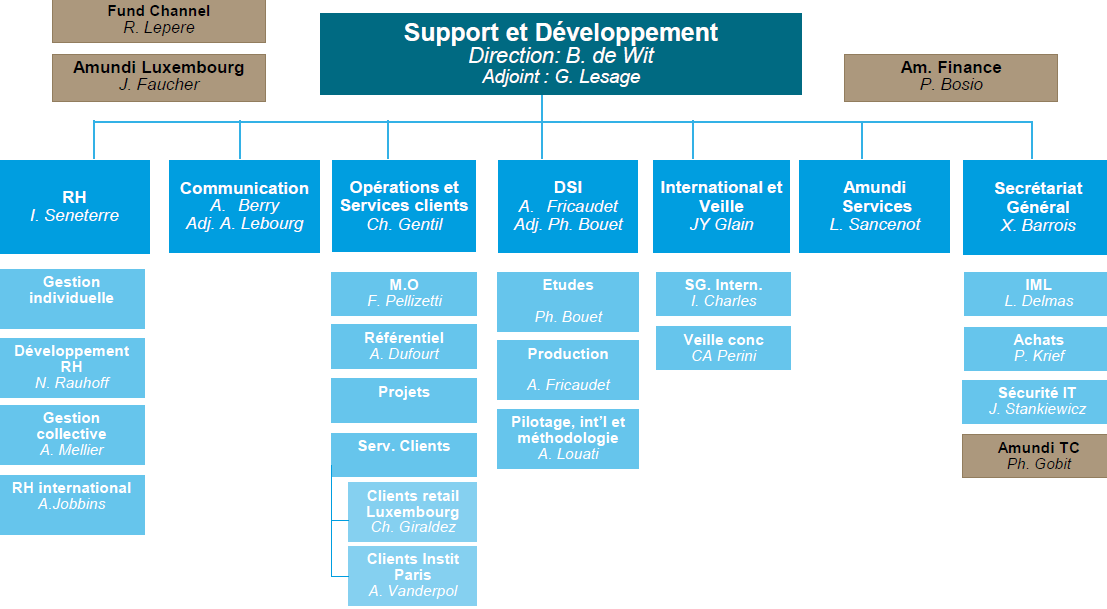
\includegraphics[scale=0.7]{IMG/orga3.png} 
\end{itemize}
\subsection*{}
L'organisation d'Amundi est globale avec une stratégie définie au niveau de l’ensemble du groupe. Cette stratégie se décline localement en fonction des spécificités de chaque pays dans lesquels le groupe est implanté. Les pays ayant le statut de plateforme globale sont les suivants : Japon, Hong-Kong, Singapour, Italie, Grande-Bretagne, Etats-Unis. Le responsable de chacun de ces pays est membre du Comex.
\section{\textbf{ Conformité}}
\subsection{Organisation}
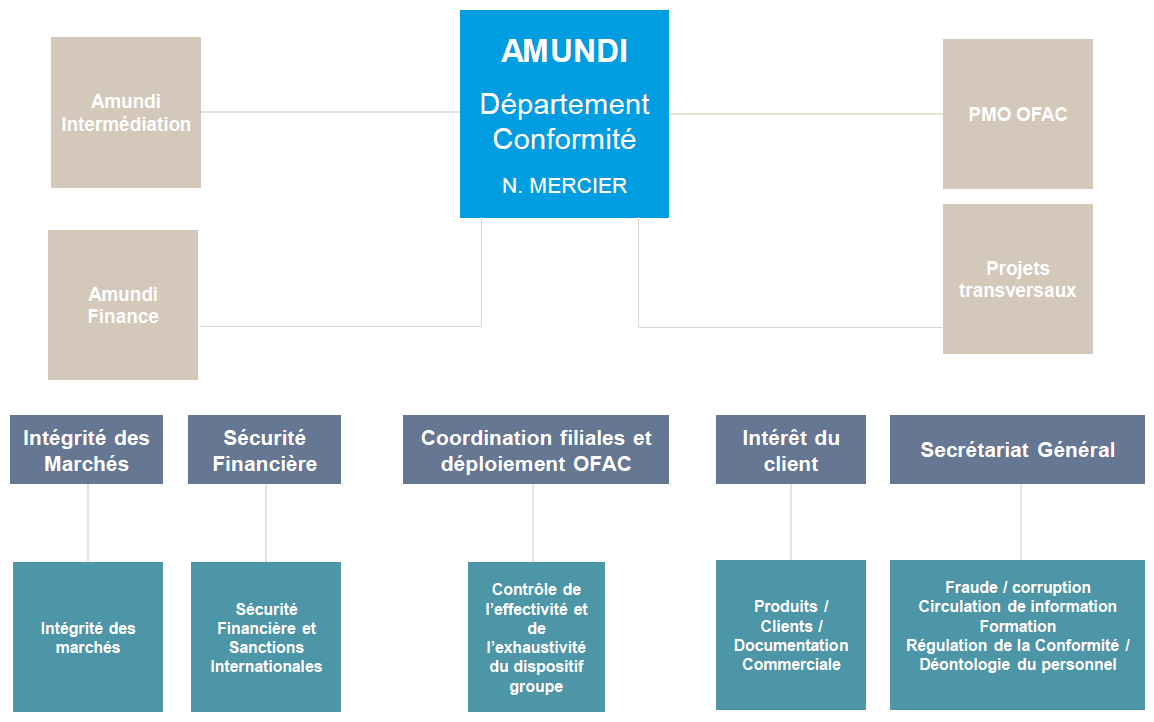
\includegraphics[scale=0.7]{IMG/cpl.png}
\subsection{Missions} 
\subsubsection{Intégrité des marchés}
Dans l’organisation d’Amundi les activités de gestion et de négociation sont séparées. Le service de RTO et d’exécution pour compte de tiers est confié à Amundi Intermédiation qui offre également ses services à des clients externes. Le dispositif de contrôle reflète cette organisation. Ses missions sont diverses : \newline
\begin{tabular}{p{.6\textwidth}p{.6\textwidth}}
\flushleft 
\begin{itemize}
\item Abus de marché
\item Délit d’initiés
\item Horodatage/ Pré et Post-affectation des ordres
\item Market Timing et Late trading
\item Erreurs / Suspension / Recalcul des Valeurs liquidatives
\item Cross Trade
\item Swing Pricing
\item Autoconsommation
\item OTC Structurés-Emissions
\item Sélection/Paiement de la recherche
\item Conflits d’intérêts: indépendance vis-à-vis du groupe Crédit Agricole / protection de l’intérêt du client
\item Reporting et déclarations statutaires et réglementaire :
\begin{itemize}
\item Franchissement de seuil
\item Vente à découvert
\item Reporting aux émetteurs
\item Reporting BHCA
\item POTAM
\end{itemize}
\end{itemize}

& \flushright
\begin{itemize}
\item Manipulation de cours
\item Best Execution
\item Best Selection
\item Fair allocation
\item Egalité de traitement
\item Demandes Régulateurs
\item Reporting des transactions (RDT)
\item Reporting réglementaires
\item Gestion des Commissions de Courtage Partagées
\end{itemize}

\end{tabular}

\subsubsection{Sécurité Financière et les Sanctions Internationales}
La sécurité financière lutte contre les embargo, le blanchissement d'argent en identifiant les sources de provenance de l'argent à souscrire dans un fond. Ses principales missions sont :\newline 
\begin{tabular}{p{.6\textwidth}p{.6\textwidth}}
\flushleft 
\begin{itemize}
\item Définition des politiques Groupe
\item Veille réglementaire
\item Analyse des Sanctions
\item Revue des clauses AML dans les contrats
\item Avis et Position de Conformité
\end{itemize}

& \flushright
\begin{itemize}
\item Contrôle permanent Sécurité financière
\item Criblage LCB/FT et Sanctions Internationales
\item Contrôle KYC/KYB
\item Due diligences
\item Reporting réglementaire, EWRA …
\item Escalade et remontée des alertes
\end{itemize}

\end{tabular}

\subsubsection{Produits / clients / Documentation Commerciale}
S'occupe de la conformité des documents de promotion et de commercialisation d'un produit. C'est le service chargé de vérifier q'un document est exacte, claire, et non trompeur. Ses missions sont entre autres : \newline
\begin{itemize}
\item Validation des nouveaux produits et des nouvelles offres
\item Communication Client (Validation documentation commerciale et marketing)
\item Validation des contrats Clients
\item Contrôle des sites Internet Amundi
\item Suivi et consolidation des réclamations Clients
\item Formation Services Clients / Commerciaux / Marketing
\end{itemize}
\subsubsection{Secrétariat Général}
C'est le service en charge des thématiques fraude, corruption, et la déontologique des salariés. Ses missions sont :\newline
\begin{tabular}{p{.6\textwidth}p{.6\textwidth}}
\flushleft 
\begin{itemize}
\item Prévention de la Fraude interne / Corruption
\item Suivi des Initiés Permanents et Ponctuels
\item Barrières d’informations (Circulation des informations priviliégiées)
\item Informations Confidentielles
\item Formation Conformité/ Professionnelle (Certification AMF/carte démarcharge).
\item Conformité des informations aux porteurs : rapport annuel
\end{itemize}
& \flushright
\begin{itemize}
\item Prévention Conflits d’intérêts
\item Déontologie du personnel / Ethique
\item Code de conduites
\item Formalisation des avis de confomité (hors OFAC)
\item Dispositif d’enregistrement
\item Conformité des délégations : Internes /Externes
\item Classification MIF des avantages et rémunérations (Inducement)
\end{itemize}
\end{tabular}

\subsubsection{Support et Coordination aux Filiales}
Fait parti de la conformité et s'occupe de la coordination de la communication entre les différentes entités.
\begin{itemize}
\item Monitoring des risques de non-conformité
\item Consolidation des cartographie de risques de non-conformité
\item Consolidation et monitoring des plans de contrôles
\item Consolidation des EWRA
\item Accompagnement des nouvelles sociétés dans le dispositif
\item Accompagnement des filiales pour décliner les politiques en procédure locale en se basant sur les travaux du pôle expertise / veille réglementaire / procédures
\end{itemize}
\subsubsection{Projets Transversaux}
\begin{itemize}
\item Projets / Organisations Conformité
\item Reportings Groupe
\item Plan de contrôle Conformité
\end{itemize}
\subsubsection{Amundi Finance}
Amundi Finance est l’entité d’Amundi spécialisée dans l’émission de garanties d’OPCVM (garantie de capital et/ou de performance), en particulier les fonds garantis distribués dans les Réseaux Partenaires. Amundi Finance est rattachée au Pôle Support et Développement.

Afin de pérenniser et développer la promotion de fonds garantis, Amundi Finance s’est dotée des capacités opérationnelles et financières nécessaires à la compensation et la collatéralisation de l’ensemble des swaps OTC des fonds garantis.
\newline
Lors de la conclusion des contrats de swaps de performance, Amundi Finance s’intercale entre chaque OPCVM garanti et sa ou ses contreparties de swaps.
Cette centralisation des contrats d’échange permet de compenser dans un cadre juridique sûr les positions créancières et débitrices face à une même contrepartie. C’est également un moyen de simplifier la gestion et le suivi opérationnel de la collatéralisation (appels en garantie espèces quotidiens) en regroupant au sein d’une seule entité, Amundi Finance, l’ensemble des opérations face à une dizaine de contreparties. Amundi Finance gère ainsi en une dizaine d’appels de marge quotidiens ce qui, si l’on avait opté pour une collatéralisation directe entre les fonds et leurs contreparties, aurait représenté plus de 250 opérations par jour.\newline Ce dispositif permet à tous, nos contreparties comme Amundi de réduire ses propres risques et d’améliorer la compétitivité des formules proposées à nos investisseurs.
\begin{itemize}
\item Conformité du développement d’Amundi Finance
\item Monitoring et plan de contrôle d’Amundi Finance
\item Conformité du développement de l’activité de structuration et de couverture des produits structurés (Solutions Structurées)
\end{itemize}
\subsubsection{Amundi Intermédiation}
Détenue par Amundi Finance et Amundi, Amundi Intermédiation est une société Prestation de Service en Investissement spécialisée dans l’activité de RTO (Réception et Transmission d’ordres ou d’Exécution d’ordres pour compte de tiers), agréée par le CECEI le 26 mai 2005. Elle intervient pour le compte des portefeuilles gérés par les équipes d’Amundi Group tant à Paris qu’à l’International, mais également pour des clientèles tiers tel que compagnies d’assurance ou Banques de Gestion Privée. 
Cette plateforme de négociation rassemble les différents spécialistes qui interviennent en aval du processus des décisions d’investissement prises par les gérants d’Amundi Group. 
Amundi Intermédiation se positionne comme un acteur essentiel de ce processus, en offrant différentes prestations à valeur ajoutée.
\begin{itemize}
\item Monitoring de la négociation
\item Best execution / Best sélection des contreparties
\item Abus de marché / Front Running
\item Egalité de traitement et Fair Allocation
\item Administration des flux de paiement de recherche
\item Gestion des cartes professionnelles
\end{itemize}

\subsubsection{Plan de Remediation OFAC}
\begin{itemize}
\item Pilotage du Programme « Plan de Remédiation OFAC » pour le Groupe Amundi
\item Programme composé de 7 Projets et 118 actions à réaliser sur 3 ans, durée du Programme
\item Gestion du Projet couvrant les sujets relatifs aux Données et à leur exploitation (KYC, Criblage, Filtrage)
\item Coordination du plan d’Action Amundi avec la Direction du Programme CAsa
\end{itemize}

\newpage
\section{\textbf{Conformité et Equipe IT}}
La Direction de la conformité veille au respect des lois, règlements, codes de bonne conduite et règles internes propres à l'activité. Son objectif est d'éviter tout abus de marché potentiel (directive sur les abus de marché), de mener des contrôles de luttes anti blanchissement et aussi de contrôler les franchissements de seuils.
La conformité réalise ses missions de contrôles grâce à l'outil \textbf{ACTIMIZE}.
\subsection{Equipe IT : mon équipe}
Rattachée à la direction informatique du groupe Amundi, l’équipe études informatique Compliance est dédiée aux besoins informatiques et au maintien des applications de la ligne métier Conformité (Sécurité financière, Intégrité des marchés financiers…).\vspace{0.3cm} \newline
L’équipe est composée de 6 personnes, développeurs et maîtrises d’ouvrage disposant de profil mixte informatique, et intervient dans la gestion et le développement  des outils informatiques notamment l'outil \textbf{ACTIMIZE}.
C’est au sein de cette équipe que j’ai évolué pendant mon stage.\vspace{0.9cm}  \newline 
\begin{center}
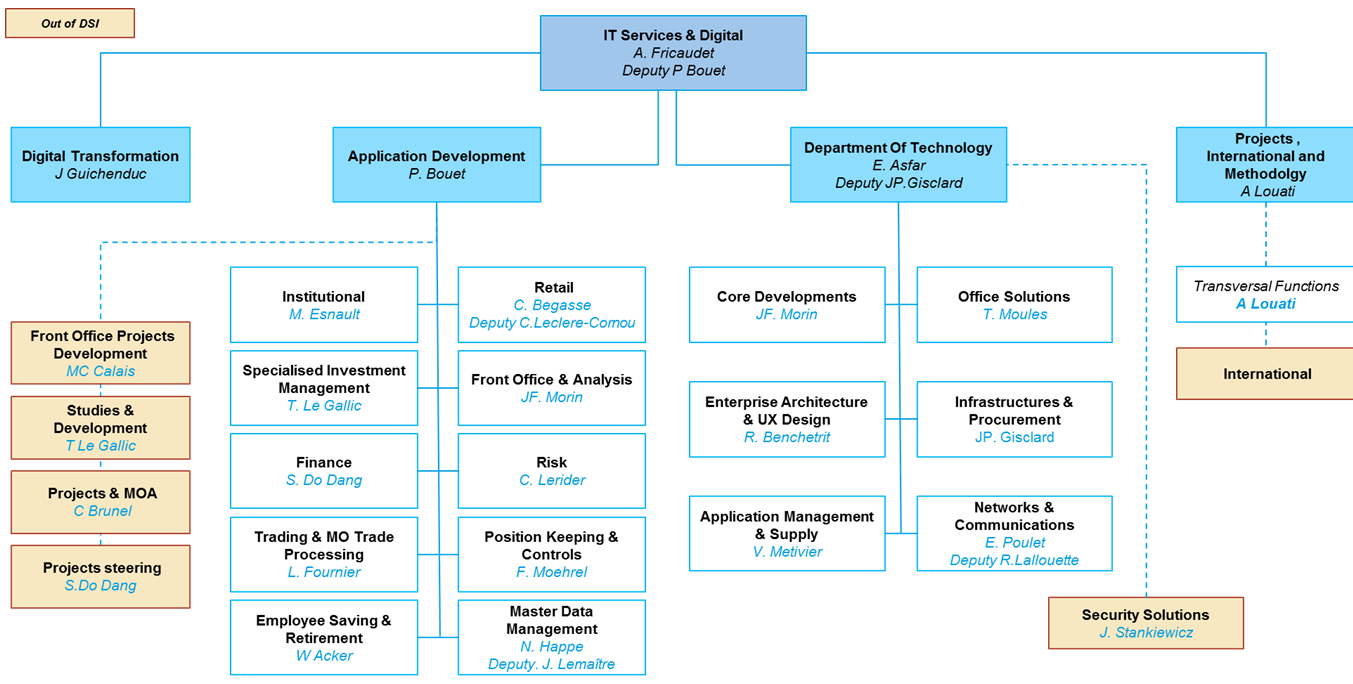
\includegraphics[scale=0.7]{IMG/it.png}
\end{center}

\newpage
\section{\textbf{ACTIMIZE}}
Actimize est un outil de contrôle contre les blanchissements et les abus de marché. C'est un outil propriétaire commercialisé par la société NICE Actimize. Il se décompose en deux parties :
\subsection{Actimize AML}
Actimize AML (Anti Money Laundering) est une partie d'actimize consacrée au traitement des informations des clients d'Amundi afin de lutter contre le blanchissement d'argent. 
Actimize AML est installé sur une plate-forme unique et centralisée qui traite toutes les entités / filiales. De cette façon, toutes les informations sont contrôlées / traitées avec la même rigueur pour toutes les entités d'Amundi. Les données sont traitées globalement; Seules les alertes sont ventilées par BU pour respecter le principe de confidentialité des informations entre chaque entité.\newline
Les contrôles effectués sont entre autre :
\begin{itemize}
   \item Contrôle PEP : vérifier que la personne n'est pas une personne exposée politiquement 
   \item Contrôle sur les données caractéristiques du client (ancien terroriste, personne recherchée ...)
\end{itemize}   
Actimize AML produit des alertes qui sont le résultat des calculs des modèles, Ils permettent l'optimisation du contrôle en attirant l'attention du compliance officer sur des cas spécifiques sur lesquels se concentrer:
\begin{itemize}
\item Le nom d'un client, semblable à celui figurant sur une liste de sanctions;
\item Souscriptions / opérations de rachat en très courte période avec des montants similaires;
\item Opération insolite de souscription / rachat pour un client.
\end{itemize}

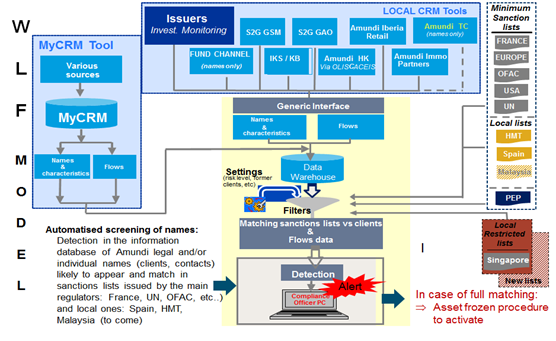
\includegraphics[scale=1]{IMG/aml.png} 
\begin{center}
\textbf{Architecture Actimize AML}
\end{center} \vspace{0.3cm}
\subsection{Actimize MAD}
Actimize MAD(Market Abuse Directive) est la deuxième grosse partie d'actimize dédiée à la lutte contre les abus de marché potentiels. Il permet de mener des contrôles sur les données de marché, des surveillances commerciale, afin de lutter contre les manipulations de marché, les fraudes et plus encore.
C'est un outil permettant de :
\begin{itemize}
\item Vérifier les opérations, les transactions, les exécutions, évitez l'arbitrage entre les portefeuilles en contrôlant les transactions courantes et le respect de la conformité (nécessite une autorisation préalable des gestionnaires de fonds aux agents de conformité)
\item Vérifier que les exécutions partielles sont bien réparties proportionnellement aux ordres initiaux entre les portefeuilles pertinents afin de respecter l'égalité des détenteurs
\item Détecter les réaffectations non volontaires d'actifs en raison généralement d'erreurs d'imputation (transfert de gain ou de perte sur un autre portefeuille) et non autorisées par la Conformité
\end{itemize}
\newpage Le contrôle consiste à :
\begin{itemize}
\item s'assurer qu'aucun ordre direct n'a été négocié par un gestionnaire de fonds avec un courtier ou une contrepartie, à quelques exceptions près.

\item assurer la traçabilité et la pré-allocation des ordres envoyés à la voix à la table de négociation par les gestionnaires de fonds
\end{itemize}
\vspace{0.6cm}
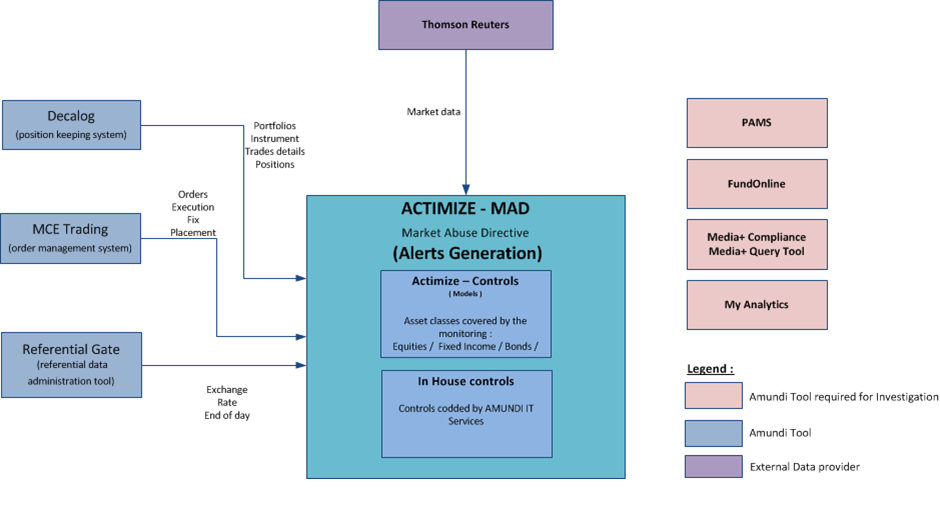
\includegraphics[scale=1]{IMG/mad.png} 
\begin{center}
\textbf{Architecture Actimize MAD}
\end{center}

\newpage
\section{\textbf{Migration Ant vers Maven}}
Maven et Ant sont deux outils de contruction de projets. L'outil Actimize est à la base un projet Ant, et l'objectif était de le migrer vers Maven afin de l'améliorer d'avantage. Le builder Maven fournit des moyens de configurations plus simple et des fonctionnalités que Ant ne possède pas.
\newline
L'origine du besoin de migrer Actimize de Ant vers maven est que le projet Actimize regroupe différents projets, sous Ant chaque projets avaient son propre fichier de compilation ce qui ne permet pas l'échange de JAR entre les projets, maven permet de répondre à ce problème car Maven télécharge les différents plugins dont il a besoin et les installe dans le répertoire maven/repository. Ainsi, les librairies téléchargées peuvent être utilisées par les différents projets.
\vspace{0.3cm}\newline
Un autre point positif de cette migration est que le system de build Maven répond aux problématiques liés au déploiement des applications. En effet, étant donné que mon équipe doit gérer plusieurs environnements : dev, recette, pré-production, production, ils passaient par des scripts pour le déploiement, ce qui revenait à effectuer les mêmes actions à chaque génération et à les adapter pour chaque projet, or Maven permet de pâlier à ces contraintes et d'uniformiser les déploiements.
\newline Un autre facteur de cette migration est l'écriture des tests unitaires (je détaillerai un peu plus ce point dans la section 0.5.2).
\subsection{Organisation du projet}
Ce projet était avant tout un travail d'équipe. Pour gérer au mieux notre projet, nous avons eu recours à différents outils :
\begin{itemize}
\item Jira \vspace{0.3cm} \newline 
C'est un système de suivi de bugs, et aussi un système de gestion de projet. Au cours de ce projet, jira nous a surtout servi de system de gestion et de suivi de tâches de chaque membres de l'équipe. On s'en servait notamment pour l'assignation d'une tâche à un membre de l'équipe, et une fois qu'un membre se voit assigner une tâche, il sera chargé de réaliser la tâche mais également de mettre à jour son état d'avancement à travers l'outil jira à l'aide d'un Kanban (TODO, IN PROGRESS, IN REVIEW ...) afin de permettre aux autres membres du groupe de voir son état d'avancement.
\newline  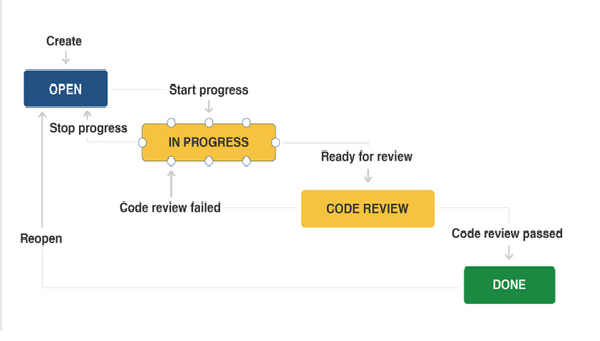
\includegraphics[scale=1]{IMG/ejira.png} \vspace{0.2cm}\newline
Cet outil nous permettait également, de suivre les étapes d'intégration d'une fonctionnalité ou la correction d'un bug jusqu'à la livraison en production. En effet, dès lors qu'un ticket passe en Review, il est pris en charge par un membre de l'équipe pour tester et vérifier que tout marche bien, ensuite il mettra le ticket à jour pour passer en production ou pour d'avantage de tests. Ainsi les livraisons concernent uniquement les tickets avec un statut <<done>>. C'est un outil qui nous a permis à moi, ainsi qu'à toute l'équipe d'être au même niveau d'information durant tout le projet.\vspace{0.1cm}\newline 
\begin{center}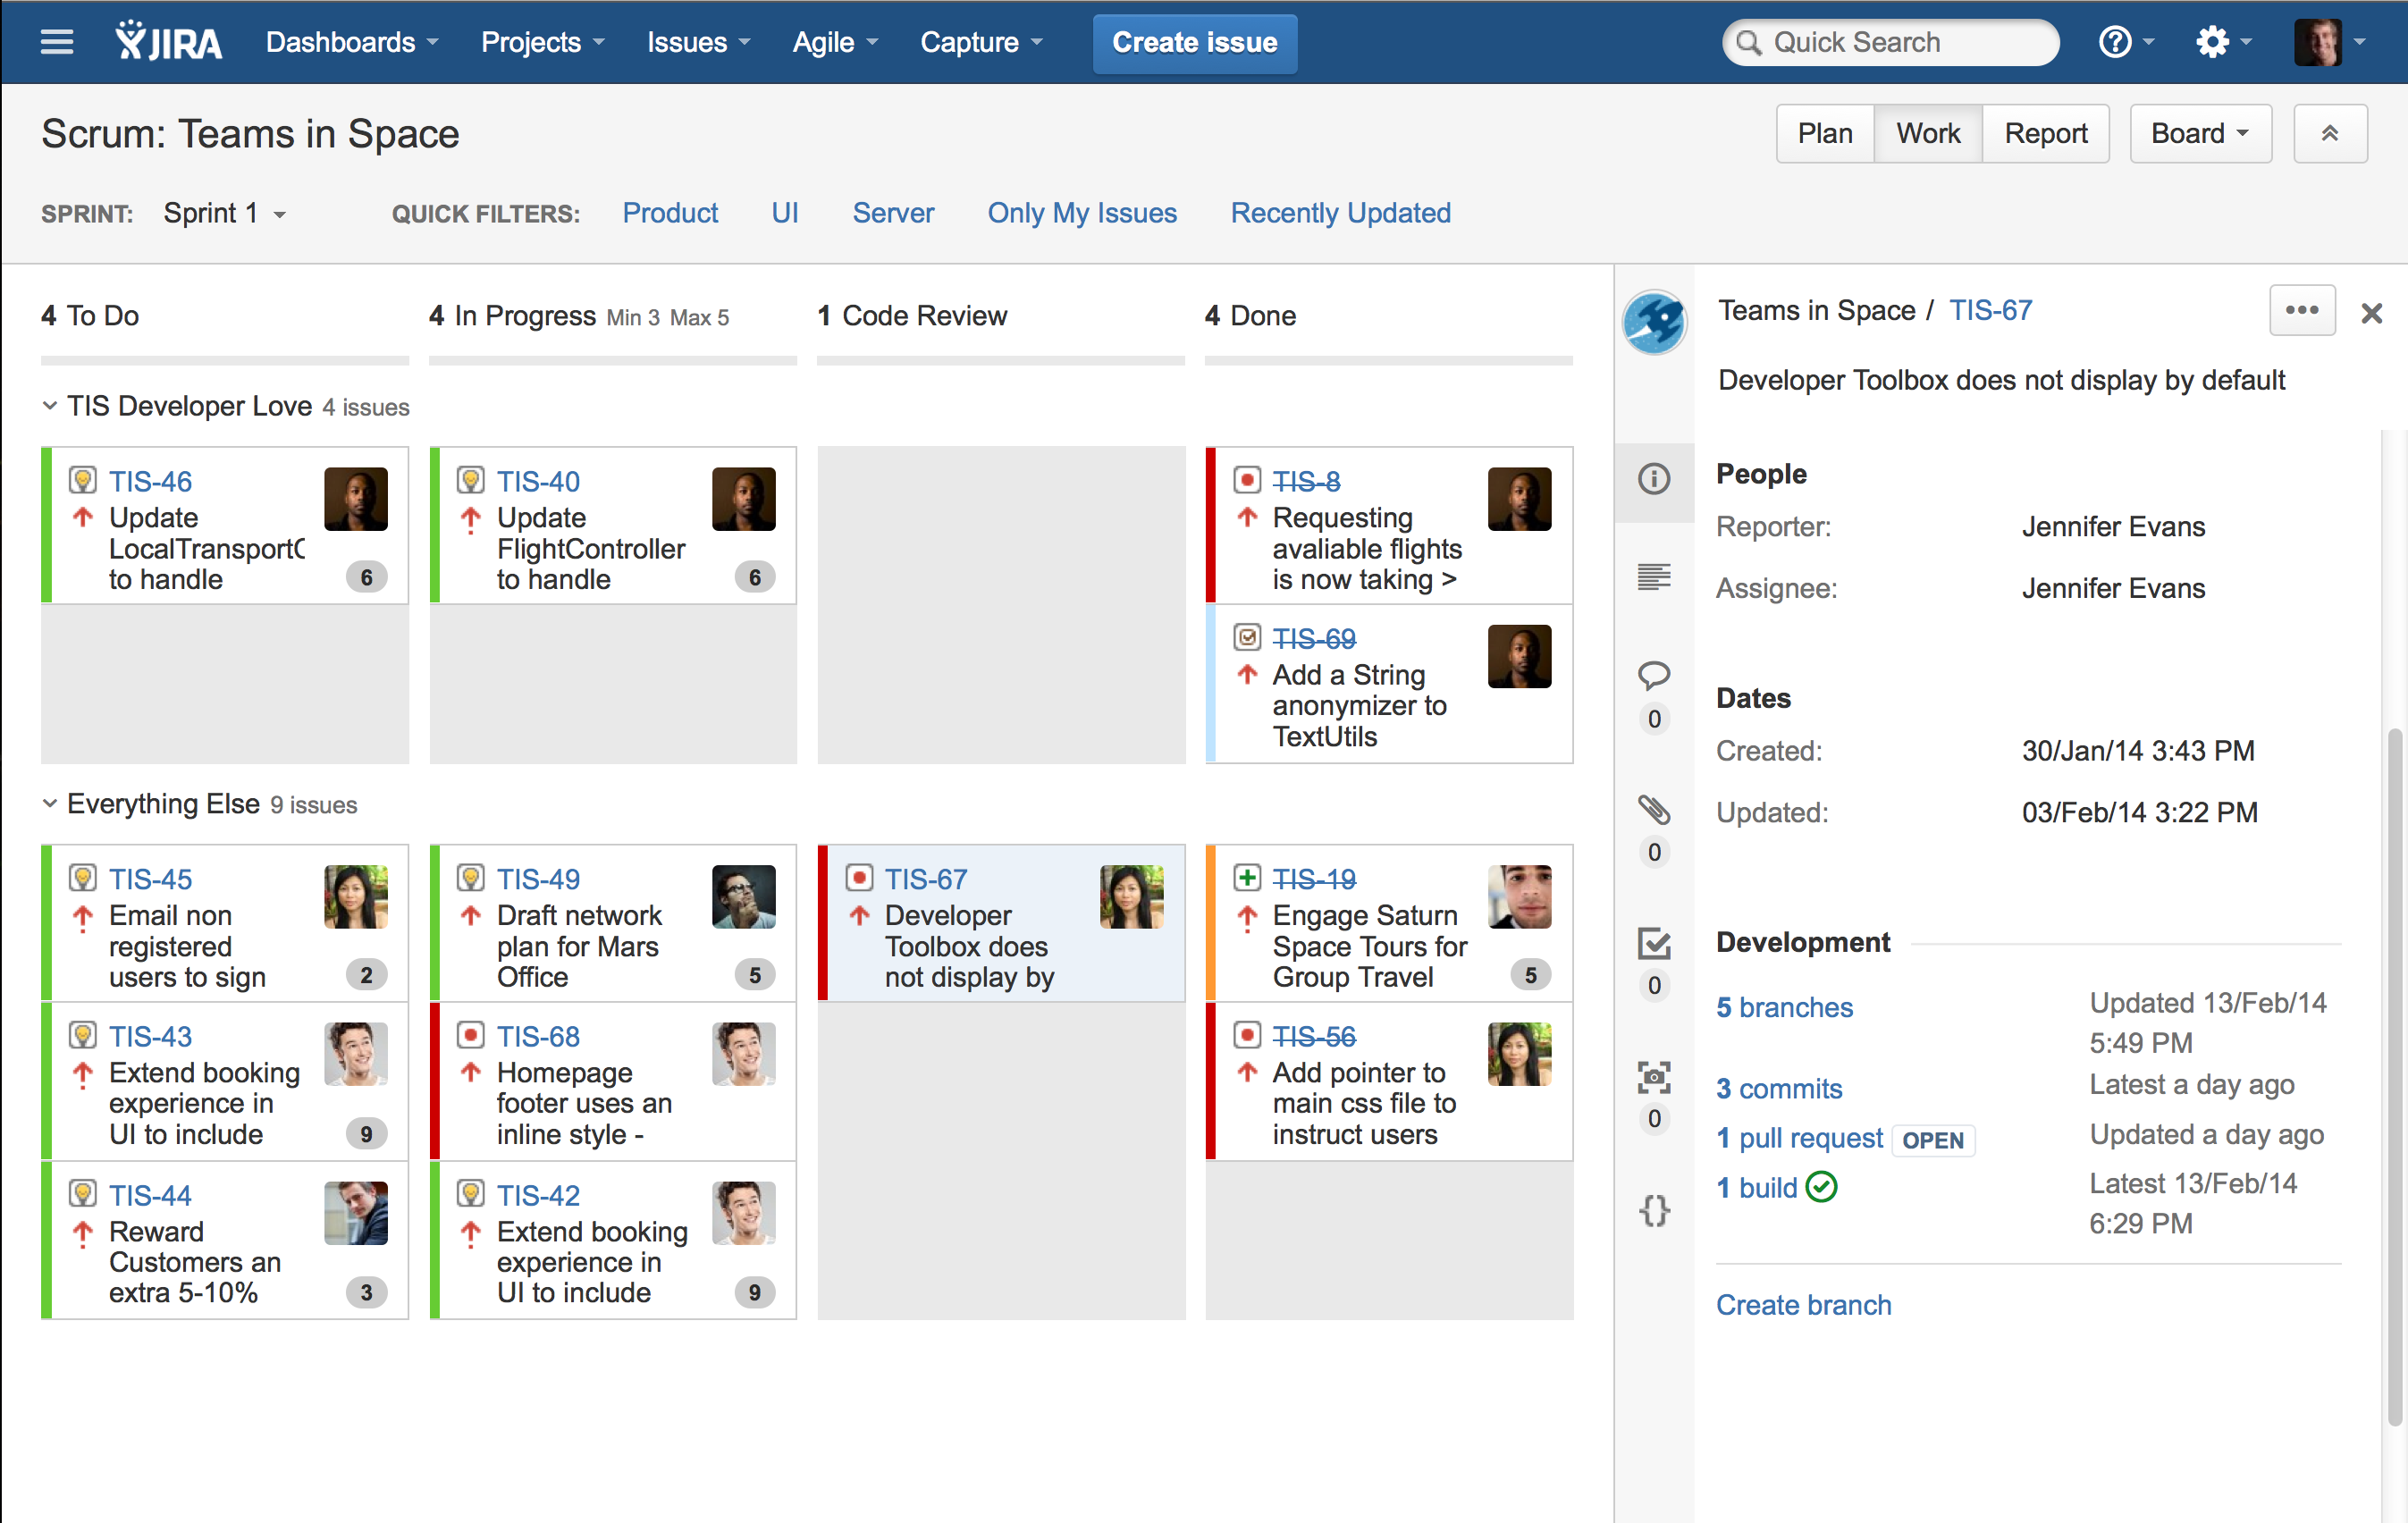
\includegraphics[scale=0.2]{IMG/jira.png}
\end{center}
\item GitHub \vspace{0.3cm} \newline
C'est un outil permettant de faire du versioning de code et du travail collaboratif. En effet le projet Actimize est disponible sur un répertoire GIT, ce qui nous permettait de travailler tous en même temps sur le projet.\vspace{0.3cm} \newline Afin de mieux gérer nos développements, avant le début de chaque dev, on créait une branche à partir de la branche dev, ou de la branche master, sur laquelle on effectuait nos développements et/ou nos modifications afin d'éviter de travailler tous en même sur une même branche. Une fois nos dev terminés, on faisait ensuite une fusion avec la branche principale pour réunir nos travailles et cela grâce à Github.
 On faisait donc un push à la fin de chaque développement avec des messages de commit portant le nom du ticket jira et l'intitulé de la tâche afin d'avoir un dépôt clean et de pouvoir facilement résoudre les problèmes. Github nous a également permis, à travers ces nombreuses fonctionnalités, dans nos développements, la possibilité de revenir sur un commit, de faire un checkout après une modification, permettre de voir la différence entre ce qui existe sur notre repository et ce que nous avons en local...\vspace{0.3cm} \newline  Avant ce stage, j'ai eu l'occasion d'utiliser GIT à travers nos projets d'études, mais ce projet m'a permis de réaliser l'importance de chaque détails(message de commit, nombre de commit, rebaser les commits...)\vspace{0.5cm}\newline 
  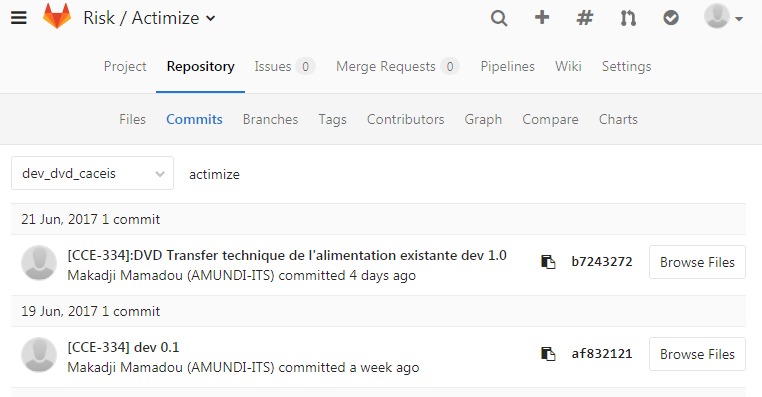
\includegraphics[scale=0.7]{IMG/git.png} 
\item Nexus \vspace{0.3cm} \newline Nexus est un système gestionnaire de livraisons. Cet outil nous a principalement servi pour la livraison de nos différentes versions sur les différents environnements.
\item Confluence \vspace{0.3cm} \newline
L'outil Confluence sert de base documentaire pour toute l'équipe. Il regroupe les documentations sur les différents outils existants, mais aussi des documentations techniques.
\end{itemize}
Outre les outils qui nous ont beaucoup aidé a bien gérer notre projet, nous avions aussi des réunions d'équipe chaque Mardi. Le but de ces réunions était d'avoir une vision de l'état d'avancement de chaque membre de l'équipe, les problèmes rencontrés, faire un état des lieux des différents projets , diffuser de l'information pour traiter collectivement ... \newline
J'avais également des points avec mon tuteur sur les parties liées au métier  afin d'acquérir des compétences générales sur le métier de la Conformité en finance. 




\subsection{Mes missions}
Durant mon stage, j'ai été amené à réaliser plusieurs missions qui sont entre autres : \newline
\subsubsection{Le Refactoring de code}
Ma première mission consistait à faire le refactoring de code des différents projets. L'objectif de cette mission était d'améliorer la qualité du code existant sans que cela ne modifie le comportement fonctionnel de l'application. Il s'agissait là de parcourir les différents projets, trouver les classes et les méthodes non utilisées dans le projet afin de les supprimer, optimiser le code en supprimant les imports non utilisés, améliorer la lisibilité du code en épurant les  morceaux de code présents en commentaire dans le projet.\newline
L'avantage de cette première mission est que ça m'a permis d'apprendre à améliorer du code sans vraiment changer son comportement, et aussi, grâce à cette mission, j'ai pu parcourir tous le code source des différents projets, ce qui m'a permis de me familiariser avec le code existant.
Un autre avantage de cette mission c'est que ça m'a permis de connaitre d'avantage de raccourcis clavier sous Eclipse, ce qui m'a permis de réaliser un gain de temps énorme durant cette mission.\vspace{0.3cm}\newline
La connaissance de ces raccourcis m'a par exemple permis de faire quelques tâches assez rapidement, exemple :
\begin{itemize}
\item Pour supprimer automatiquement tous les imports non utilisés dans une classe, j'ai pu le faire directement grâce à mon IDE au lieu de parcourir manuellement toutes les classes pour trouver les imports non utilisés et les supprimer, ce qui, au finale aurait pris énormément de temps.
\item Pour connaitre le nombre de fois qu'une méthode est utilisée et les classes dans les lesquelles elle est utilisé dans tous le workspace. 
\end{itemize}
\subsubsection{La Gestion des exceptions}
Ma deuxième mission consistait à bien écrire et  corriger l'utilisation des exceptions dans les différents projets et de centraliser les messages d'exception dans le projet en commun afin que les autres projets puissent les utiliser (amélioration et meilleure lisibilité du code). Une exception est une erreur se produisant dans un programme qui conduit le plus souvent à l'arrêt de celui-ci. En effet, dans les différents projets, l'écriture des exceptions ne nous permettait pas de savoir exactement quel type d'exception a été capturé et souvent les exceptions étaient capturées, mais pas levées, ma mission était donc de réécrire ces exceptions afin de les affiner pour que l'on puisse savoir exactement quelle exception a été capturer et assurer qu'on lève bien  l'exception. J'ai dans un premier temps identifié les lignes de codes pouvant générées une exception, puis j'ai écrit le code permettant de détecter, de traiter ces erreurs mais aussi de les lever afin d'avoir une meilleure gestion des erreurs dans tout le projet.  

\subsubsection{Développement de fonctionnalités} 
Durant cette mission j'ai été amené à ajouter des fonctionnalités dans le code existant notamment sur les parties liées au traitement des batch. En effet, nous avons au sein du projet des batch qui génèrent des traitements au quotidien, ces traitements sont entre autre la génération et le traitement de fichiers, l'envoie de ces fichiers à d'autres entités, la sauvegarde sur le serveur ... Durant cette mission, j'ai travaillé plus précisément sur un batch qui génère un fichier chaque jour contenant des données confidentiels, crèe un zip du fichier afin de l'envoyer soit par mail, soit par SEF (envoi entre serveurs) aux entités concernées, puis archive ces fichiers. J'ai été amené à ajouter une fonctionnalité (en java) qui permet de supprimer les fichiers zip une fois envoyé, et aussi de changer le répertoire source de ces fichiers sur le serveur, et pour finir je devais rajouté une fonctionnalité permettant de vérifier que les fichiers générés ne sont pas vides et si c'est le cas ma fonctionnalité devra générer un warning avant l'envoi du fichier.\vspace{0.5cm}\newline
J'ai également développé un job de traitement qui n'existait pas chez nous, mais dans une autre équipe. C'est un job de traitement de positions et mouvements. Etant donné que notre équipe utilisait ce traitement avec des possibilités limitées(notamment le fait que ce traitement soit effectué sur les données d'une base de données externe), l'idée était donc créer ce même traitement chez nous afin de pouvoir gérer facilement nous même les données. Je suis donc intervenu sur la création de ce traitement pour l'ajouter à l'existant. Au cours de ces développements, j'ai utilisé notamment du SQL pour la gestion des données dans notre base, la réécriture du code existant en ksh vers du code SQL, puis du JAVA pour exercer à chaque fois les traitements sur nos données, puis extraire les résultats dans des fichiers au format(.csv). L'utilité de ce nouveau job est de pouvoir facilement gérer les données sans passer à chaque fois par une autre équipe, lorsque l'on souhaite ajouter, modifier ou supprimer une ou plusieurs données de contrôles.  
\subsubsection{Amélioration de la qualité du code}
Nous avons à travers les différents projets, beaucoup de fonctionnalités développés en fonction de ce que proposait les anciennes version du JDK (Java Development Kit), mon rôle dans cette mission a été de réécrire ces fonctionnalités afin  d'utiliser uniquement le JDK 7 qui offrait plus de possibilités que les anciennes versions. Pour mener à bien cette mission, j'ai d'abord regardé les améliorations que dispose le JDK 7 par rapport aux anciennes versions. J'ai donc réaliser les améliorations envisageables grâce à cette nouvelle version, elle permettait entre autre la gestion automatique de fermeture des ressources ce qui est très important dans un projet tel que le nôtre (avant que je ne réécrive ces classes la gestion des ressources dans le projet était gérée  manuellement, ce qui nous assurait pas qu'on gérait convenable l'utilisation des ressources), elle permet également d'améliorer l'utilisation des collections en java comme éviter la duplication de la déclaration des types paramétrés et plein d'autres choses. La finalité de ces améliorations était de mettre le projet dans les normes.
\subsubsection{Ecriture des tests unitaires}
C'est l'une des missions les plus intéressante que j'ai eu à faire pendant mon stage. L'écriture des tests est très important dans un projet, car les tests permettent
de s'assurer que tout fonctionne bien et surtout qu'elle fonctionne dans toute les situations possibles. Avant cette mission, le projet actimize n'avait pas de test car au lancement du 
projet l'équipe ne pratiquait pas de TDD (Test Driven Development ou en Français Développement Dirigé par les Tests). Je devais donc écrire les tests de tout le projet.
\vspace{0.3cm} \newline Pour mener à bien ces tests, j'ai utilisé le framework de test JUnit.\newline
J'ai dans un premier temps ajouter les dépendances de JUnit dans le projet, puis j'ai commencé à écrire quelques tests, mais je me suis très vite rendu compte que pour faire des tests de qualité 
et surtout pour pouvoir tester toutes les méthodes, il me fallait d'autres framework de test car JUnit n'offre pas beaucoup de possibilités.
J'ai donc rajouté les frameworks :
\begin{itemize}
\item Mockito \vspace{0.3cm} \newline
C'est un framework de tests très puissant car il permet notamment de simuler le comportement d'un objet et offre plusieurs méthodes de tests. Je me suis donc documenté sur ce framework qui jusque là était nouveau pour moi en allant lire la documentation officielle du framework, puis j'ai commencé
à me familiariser en lisant des tutoriels sur internet, et en réalisant des tests basiques.
L'un des plus gros avantage de ce framework c'est qu'il consomme moins de ressources pour les tests car il simule une doublure de l'objet à tester.
\item AssertJ \vspace{0.3cm} \newline
J'ai également utilisé le framework assertJ pour plus d'assertions, car il contient énormément d'assertion que JUnit ne propose pas. En effet, le framework de test AssertJ permet de palier au problème de limitation des assertions basiques proposées par JUnit, à savoir AssertEquals et ses variantes. Parfois, il m'étais difficile de vérifier ce que je voulais par manque d'expressivité (exemple pour les listes). L'expressivité d'AssertJ est très puissante notamment sur les assertions spécifiques aux collections. AssertJ permet de vérifier également que les exceptions sont bien jetées par une méthode...\newline
En plus de proposer beaucoup d'assertions et d'être puissant, l'une des principales raison pour laquelle j'ai utilisé AssertJ est sa facilité d'utilisation et aussi l'existence de très bonnes documentations en ligne.
\end{itemize}
Une difficulté que j'ai rencontré durant cette mission est que je devais comprendre le comportement de chaque méthode à tester comme si c'était moi qui l'avait développé pour ensuite pouvoir écrire les bons tests.\newline Cette mission a été très enrichissante car ça permis de m'améliorer d'avantage dans l'écriture des tests unitaires, mais aussi d'apprendre à utiliser d'autres frameworks de tests. Dans l'avenir, je devais refaire des tests unitaires, je n'hésiterai pas à utiliser ces trois frameworks car ils sont indispensables et complémentaires.
\newpage
\section{\textbf{Mon avis sur ce stage}}

\subsection{Les apports} 
Mon stage chez Amundi m'a beaucoup apporté tant sur un plan professionnel que personnel. J'ai acquis à travers ce stage une solide expérience sur la mise en place et conduite de migrations techniques, en qualité, conception de développement informatique. Ce stage m'a permis de travailler sur un vrai projet d'envergure, et de développer 
mon aptitude à travailler en équipe.
Techniquement, ce stage m'a permis de m'améliorer d'avantage sur le développement en Java notamment sur l'écriture des tests 
unitaires (JUnit, Mockito), et les bonnes pratiques de développement (apprendre à écrire des lignes de codes plus lisibles, optimisation ...), ça m'a également permis d'avoir beaucoup de connaissances sur l'utilisation de GitHub j'ai pu apprendre beaucoup de commandes, et les bonnes pratiques pour 
mieux utiliser cet outil si précieux (mieux gérer ses commits, éviter les conflits ...), j'ai également acquis une large compétence sur comment mieux travailler avec son IDE (Eclipse).
Sur un aspect métier, ce stage m'a permis d'acquérir des compétences dans le métier de la conformité en Finance.
\subsection{Les difficultés rencontrées} 
Avant de travailler chez Amundi, je n’avais pas de connaissances particulières sur le métier de la conformité en finance, c’est pourquoi il a été difficile au début de tout assimiler. 
Une autre difficulté que j'ai rencontrée au début a été de me familiariser avec le projet sur un aspect technique, j'avais un peu de mal à comprendre le rôle et les étapes d'exécution des batch.\newline
Un autre point en terme de difficulté qu'il est important que je mentionne est l'anglais, Amundi étant une société de gestion internationale, tout était quasiment en anglais, j'ai donc réalisé que j'ai des lacunes dans cette langue mais aussi et surtout son importance.
\newpage
\section{\textbf{Conclusion}}
En définitive, j'ai effectué mon stage de fin de master 1 MIAGE au sein de l'entreprise Amundi Asset Management. Lors de ces 12 premières semaines de stage, j'ai pu mettre en pratique mes connaissances théoriques et pratiques acquises durant ma formation, notamment en programmation JAVA et SQL à travers les différents projets qui m’ont été confiés. Les connaissances acquises durant ma formation m'ont permis de mener à bien mes missions, j'ai par ailleurs pu les approfondir grâce aux nombreux conseils qui m’ont été accordés. Ce stage à Amundi m’a énormément appris sur le monde de l’entreprise, la gestion d'un projet, le travail en équipe. Il a constitué pour moi une très bonne expérience tant au niveau professionnel qu’au niveau personnel. Il m’a permis d’appliquer les méthodes informatiques que l’on m’a enseignées ces quatre dernières années, J’ai également appris à améliorer mes méthodes de travail, notamment grâce au soutien de toute l’équipe, qui m’a très bien conseillé pendant tout mon stage Enfin, je tiens à exprimer ma satisfaction de travailler dans de bonnes conditions matérielles et un environnement agréable.

\end{document}